
\section{Spatial Election}

Spatial Election is a software developed in Java by Martin Liesenberg and
Alexander D\"umont. It was created as result of an academic project during the
lecture \textit{Spatial Databases} given by Agn�s Voisard. \\

Spatial Election is implemented as a client server application. The backend is
developed in the programming language \textit{Java} and uses the database
\textit{Postgres}. The frontend site is a website, which uses \textit{HTML},
\textit{JavaScript}, \textit{SVG} and \textit{CSS} for visualization purposes.

\begin{center}\rule{3in}{0.4pt}\end{center}

\begin{figure}[htbp]
\centering
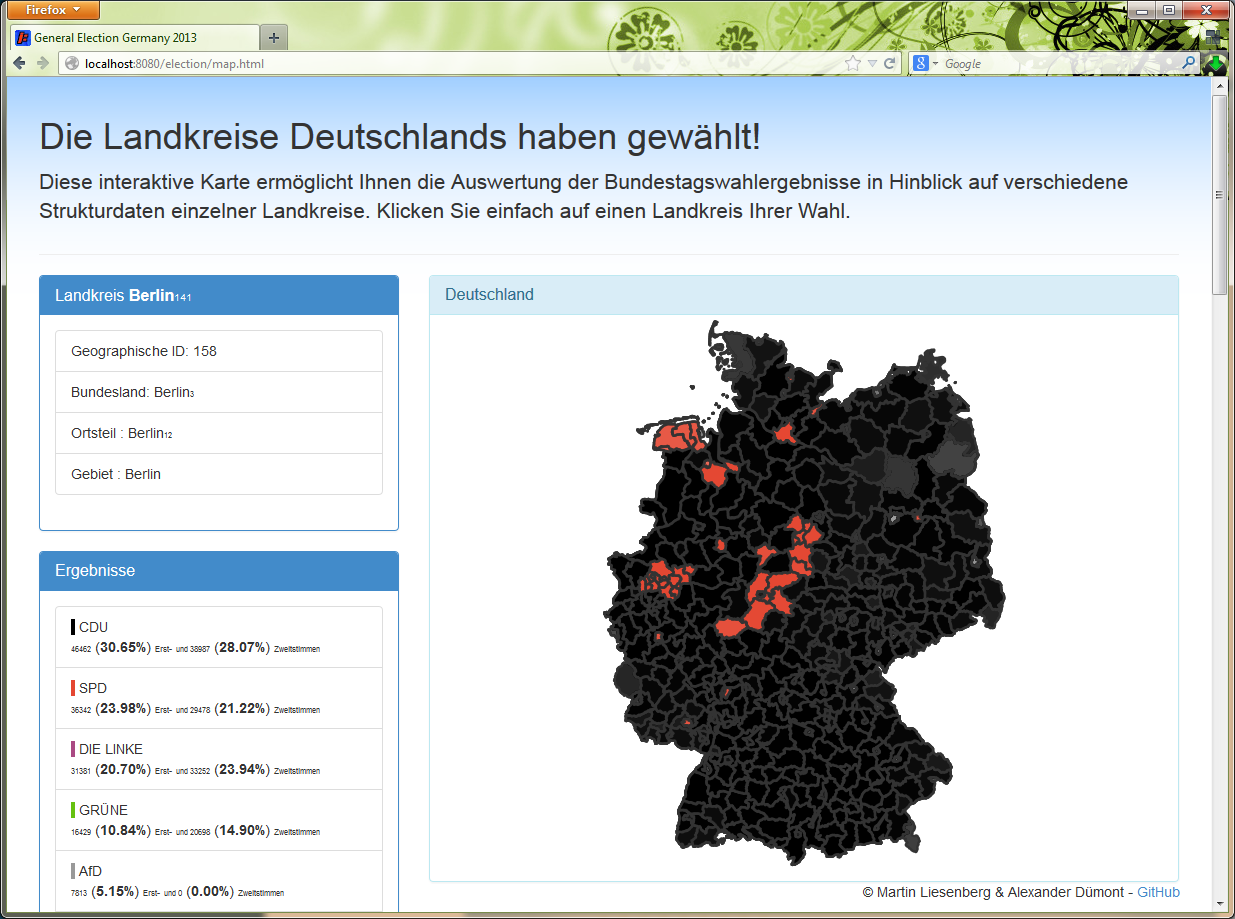
\includegraphics[width=1.2\textwidth]{../img/JKGj20F.png}
\caption{Browser Screenshot}
\end{figure}